\chapter{Introduction and Background}

\section{Introduction}

The human body is the product of a four-billion-year-old pileing-up of nanotechnological hacks, which exists because, for that four billion years, none of its ancestors died without issue; we have hijacked it and are now attempting to use it to carry us around while we compose symphonies, build telescopes, write Ph.D. theses, and generally attempt to be people as opposed to just humans. We don't really know how it works, we don't have access to the proper servicing equipment to fix it properly when it breaks, and the thing just wasn't really meant to do what we're trying to do with it. The goal of human genomics is to figure out how these things we call our bodies actually work, so that we can do more than just change the nanotechnological oil and hope for the best.

Achieving this goal is relatively difficult, because of the scale of the problem. Each human genome is about 3.2~billion base pairs, and each human has two genomes (one from each gamete). %Each of those base pairs has four possible values (\texttt{A}, \texttt{C}, \texttt{G}, \textt{T}), providing a truly untennable $3.16 \times 10^{3853183944}$ combinations.
Human brains struggle to think about a even a single billion of anything, a number so large that a one-in-a-million chance occurs on average a thousand times. Add to this the already-difficult-to-comprehend non-designed-ness of the entire system, where no part is really ``for'' anything, and you can begin to get a sense of the difficulty of the problem.

Fortunately, despite the limitations of our tiny meat brains, we are beginning to develop techniques and guiding principles for working with problems at these scales. One of those principles is that large problems can be effectively addressed by integrating across large data sets \cite{halevy2009unreasonable}. With a population now exceeding 7.5~billion individuals, humans may constitute a sufficiently large data set to begin to approach this problem \cite{talton2017economics}. However, effective tools to integrate genomic information at the scale of the human population will be required.

One of these tools will be a new type of genomic reference. Human genomics as it exists today is organized around something referred to as ``the human genome'', obtained through great effort and at great expense through the Human Genome Project \cite{powledge2003human}. There is a clear distinction in the field between the human genome, embodied by the reference genome assembly builds produced by the Genome Reference Consortium (GRC) \cite{schneider2013genome}, and differences from that reference, or genomic variation, embodied by the variant sets produced by efforts like the 1000 Genomes Project \cite{10002015global} or the Simons Genome diversity Project \cite{simons2014simons}. Even when efforts like this claim to produce genomes, they release Variant Call Format (VCF) files, or the equivalent, specifying their genomes with reference to and in the space induced by a reference genome assembly.

Unfortunately, this approach will not scale. Different projects have different notions of variable sites, and this makes combining variation data from multiple data sets difficult. Moreover, the most recent release of the GRC's human reference genome assembly, GRCh38, contains sequences for 261 ``alternative loci'', which are sequences intended to provide alternative versions of parts of other sequences in the assembly, in order to be more representative of large-scale and structural variation in the human population \cite{karolchik2014new}. These alternative loci are intended to essentially replace portions of the primary assembly for the purpose of analyzing certain genomes. The number of genomes for which this replacement ought to be performed is relatively large; the eight alternative loci for the Major Histocompatibility Complex (MHC) region, for example, were chosen to be representative of people of European ancestry \cite{horton2008variation}, so many of such people's genomes might be better represented by using one of those alternative loci than using what is in the primary assembly. Indeed, a recent study \cite{jager2016alternate} found that some alternative loci are likely to be present in 90\% or more of the individuals in some populations. However, most available variation data sets, variant calling tools, and indeed the VCF format itself, do not account for this, and instead cram all individuals into the space of the primary assembly, regardless of its appropriateness for the individuals or populations under study.

In genomic regions where these alternative loci apply, the traditional linear coordinate system, which refers to locations in peoples' genomes by the chromosome and base index in the primary assembly, begins to break down. To properly reason about such genomic regions, we need to abandon either the idea that bases in peoples' genomes correspond to bases in a reference, or the idea that references are linear.

The linear organization of the reference genome also frustrates attempts to study regions of the genome which are difficult to assemble, or which, due to sequence similarity, are very difficult to distinguish from similar regions at other locations in the genome. To facilitate analysis of the centromeres, for example, GRCh38 includes plausible synthetic linear centromere sequences \cite{karolchik2014new}. We have more precise, graph-based models of what we actually know about the centromeres, but these models cannot be indexed by linear sequence coordinates or processed by tools that expect a linear reference sequence \cite{miga2014centromere}.

I propose a nonlinear, graph-based ``Human Genome Variation Map'', or HGVM. This new type of genomic reference will eliminate the artificial distinction between the reference genome assembly---``the human genome''---and what we know about variation among the genomes of the human population. A graph-based reference can capture in a first-class way the sequence information which is currently relegated to alt loci, as well as additional variant information from sources like the 1000 Genomes Project \cite{10002015global}. A human genome variation map not giving preference to one version of a region with alternative loci over another could potentially combat allele-specific mapping bias, an effect in which alleles that match the single linear reference are easier to detect than those which do not \cite{degner2009effect}. The adoption of a unified representation of genomes will allow genomic analysis software to scale to much larger cross-dataset analyses, with a more represerntative view of individuals' genomes, allowing progress to be made in the unraveling of human biology.

\section{Background}

\subsection{How Bioinformatics Works}

% Say something about how we need to use more than one dude's worth of genomes to understand genomes, because more data is more better.

% But we can't use all umpteen jillion BAMs at once, so we need to reduce them down to something manageable, which is a graph reference.

\subsection{Reliable, Portable Cloud Computing with Toil}

% Talk about how great Toil is and how it let me do lots of the analyses in here

\subsection{Data Models with Protobuf}

% Talk about data models and protobuf

\subsection{How Genomics Works}

One piece of shared infrastructure that bioinformatics already uses is the human reference genome, which was built at great expense at the turn of the millennium and is maintained by the Genome Reference Consortium (GRC) \cite{church2011modernizing}. This reference genome assembly was originally created by stitching together actual observed pieces of DNA sequence into a single-copy haploid \vocab{golden path} representing a complete genome \cite{church2011modernizing}. Under this model, a hypothetical perfect assembly would have a single \vocab{contig}, or contiguous linear string of DNA bases, per chromosome. This naturally suggests a coordinate system: bases can be referred to by the contig they are on and their offset from the beginning of that contig.

This coordinate system is a critical piece of genomics infrastructure. It allows the reference genome to be annotated with genes and other elements. It provides the backbone to which descriptions of genomic variation are anchored. It defines the space in which genome sequencing happens, as short reads from sequencing machines are \vocab{mapped} to positions in this space. The entire field depends on this coordinate system.

Unfortunately, whenever the official human reference genome is updated, and bases are inserted or removed, the old coordinates are no longer valid on the new reference, and a period of mass confusion ensues as everyone who studies human genomics translates everything they are working on over to the new coordinate system, and then wonders whether their colleagues have done the same. Resources that aren't converted to the new system are at best lost to the field, and at worst applied inappropriately to the wrong genomic locations.

The golden path model is inextricably bound to the concept of ``the human genome''---the idea that one prototypical set of 24 chromosomes is a suitable foundation for the field of genomics. This idea has been central to human genomics, but it is not without its flaws. Putting aside the unfortunate normative implications of declaring the allele from whomever you sequenced first as ``reference'' and any alternatives from other populations as ``variant'', using a single reference genome when mapping sequencing reads leads to the well-known phenomenon of \vocab{reference bias}. Reads matching the reference genome at a variant site tend to map better and more often than those supporting differences from the reference. This reference bias affects many popular short-read aligners \cite{lunter2011stampy}. Additionally, in some genomic regions there are dramatically structurally distinct haplotypes present in the population \cite{church2011modernizing}. One example of this phenomenon is the extremely variable Major Histocompatibility Complex (MHC) region on chromosome 6. Mapping reads only against the single haplotype actually included in the assembled golden path will almost certainly make it harder to map reads from other haplotypes.

\subsection{The Release of GRCh38}

A new version of the official human reference genome, GRCh38, was recently released \cite{karolchik2014new}. In addition to marking the transition to a unified version numbering scheme across major genome browsers, this new release continues the GRC's gradual migration away from the golden path concept. Although GRCh38 is still constructed around a single (chimeric) haploid genome, the new reference assembly also provides sequences for hundreds of so-called \vocab{alt loci}---additional pieces of sequence with a specified alignment to that genome which describe some of the structurally distinct local genomic arrangements which have been observed in humans. The older GRCh37, by comparison, contained only three genomic regions with alt loci \cite{church2011modernizing}. This means that the GRCh38 assembly, taken as a whole, is fundamentally nonlinear at more than just a few problematic locations. Unfortunately, popular tools like BWA have not yet been updated to fully account for these alt loci \cite{li2014bwa}.

The new assembly also contains sequence for the centromeres---the central portions of the chromosomes, which contain extremely repetitive sequences that continue to defy conventional sequencing and assembly methods \cite{karolchik2014new}. However, these new centromere sequences are not directly derived from actual sequence observations, but are instead plausible linearizations of a series of graph-based centromere models \cite{miga2014centromere}. Unfortunately, the linear format discards much of the uncertainty information present in the graph models. Moreover, this additional sequence was found during testing to cause trouble for traditional short-read alignment pipelines, so GRCh38 also comes as an ``analysis set'' with these sequences masked out \cite{karolchik2014new}. The real problem, though, lies with the tools which cannot handle either a full nonlinear description of what we know about the centromeres, or even the placeholder linearization that GRCh38 includes.

In summary, GRCh38 both marks the continuation of a trend towards nonlinearity in the human reference and provides an example of the shortcomings of the golden path approach. Until tools can be updated to account for alt loci and centromere sequences, GRCh38 cannot be used to its full potential.
    
\subsection{Description of Human Genomic Variants}

There is no prototypical workflow for the analysis of variant data; what you do with it depends heavily on the scientific question that you are trying to answer. However, there are a few extremely common practices in the field. One of these is to store variant data in Variant Call Format (VCF) files, a column-based text format developed as part of the 1000 Genomes Project \cite{danecek2011variant}. Samples are represented by columns, and polymorphic positions in the human genome by rows. VCF files can be supplemented by an index on genomic position, but no work appears to have yet been done to also provide an index by sample; consequently, the scalability of VCF is currently limited to numbers of samples that can be scanned through efficiently \cite{danecek2011variant}.

VCF encodes individual samples' genomes by defining a series of variant sites along the length of the linear reference genome, defining a set of alternate alleles which have been observed at each site (in addition to the allele in the reference), and then indicating which alleles (in what phasing) are present in each sample at each site. This approach works extremely well for some types of variation, like single nucleotide polymorphisms (SNPs) and short indels in structurally quiet regions, but it also has shortcomings.

One problem with the VCF format is it does not define the semantics of the absence of a variant record. Does it mean that that position in the reference is known not to be variable in the population (or at least in the sampled portion of it)? Or does it mean that that location is not in the region covered by the VCF file? To solve this problem, the VCF format has been extended by Illumina to create the gVCF format, in which genotyped but nonvariant positions are also described \cite{saunders2014about}.

Another potential problem with the VCF format, at least from the point of view of people who need to read it, is that it is very featureful. The format is extensible, through the inclusion of header lines defining various fields. However, different VCF processing tools need to have different sets of fields defined in order to work. It is vital to check the fields output by one tool against those required by another. This makes VCF a worse standard, because knowing that a tool reads or outputs VCF does not substantially reduce the amount of thinking required to run it.

Furthermore, there are no fewer than three distinct syntaxes for specifying variants in VCF: the original syntax, in which alternate alleles are short stretches of sequence; a symbolic format, in which alternate alleles are mere specifications of inversion or duplication, or even references to named alleles defined elsewhere; and a breakend-based format, in which structural variants (and related sequence changes) are defined as a series of possibly-paired breakend records describing how the reference would have had to have been cut and spliced to produce the sample \cite{marshall2013variant}. Available VCF parsers do not help with integrating across or converting between these different internal formats, and some don't even support all of them. Tools written to directly extract information from VCFs without a parser library often support only one or maybe two of these formats. Furthermore, between the three different formats and the fact that different alignment parameters can induce variant callers to describe the same observed sequence as different variants, it is very difficult to compare two VCF files.

Finally, the VCF format is tightly coupled to the linearity of the reference genome. While VCF's breakend system allows the specification of complex rearrangement graphs for samples, there is no explicit support for even the alt loci of the current GRCh38 reference. For example, if one were to specify variant records on one of the MHC alt loci, there would be no way to specify phasing with variants on the main chr6, because VCF specifies records with different chromosome names to be unphased relative to each other \cite{marshall2013variant}. Furthermore, there is no way to explicitly specify that a sample uses a certain alt locus; it would be necessary to infer this from the existence of called genotypes in the coordinates of that alt. It would certainly be possible to adopt certain conventions within the existing VCF format to work around this problem---for example, we could wire the alt loci into their parent chromosomes with breakends whenever they are present. However, no such conventions are standardized for data interchange.

A graph-based approach to the description of genomic variants could alleviate several of these problems, defining explicitly when an individual matches the primary path of the reference, and expressing clearly and concisely the alt loci that an individual carries, and any variations on top of them, in a single sufficiently general syntax.

\subsection{String Compression with the Burrows-Wheeler Transform}
\label{subsec:bwt}

In part because of the shortcomings of VCF and its linear reference, I propose moving to an entirely graph-based conception of variants that incorporates them into a ``reference structure''. I propose a method for creating and mapping to graph-based reference structures, based primarily on string operations on a large collection of individual haplotypes. A single individual has several gigabases of DNA sequence; in order to combine many such haplotypes into a useful reference data structure, they need to be compressed. Thankfully, collections of haplotypes are likely to be highly compressible, since individual genomes are generally very similar to each other.

One particularly useful algorithm in string compression is the \vocab{Burrows-Wheeler Transform (BWT)}. The BWT takes strings and rearranges them for increased compressibility, by putting characters from similar contexts near each other \cite{burrows1994block}. (It is interesting to think of the BWT as defining a new, context-based coordinate system.)

The BWT operates by taking the string to be compressed (with a sentinel value ``\$'' lexicographically smaller than all other characters appended to it) and imagining all possible rotations of it \cite{burrows1994block, ferragina2000opportunistic}. Each rotation is derived from the previous one by taking the first character and moving it to the end \cite{burrows1994block}. The rotations are then sorted lexicographically, and the last characters of all the rotations become the transformed string \cite{burrows1994block}.

The BWT makes strings more compressible by grouping characters by the contexts they appear in (specifically, the strings they appear before). If two characters both appear before a suffix starting with ``andy'', they will appear near each other in the BWT. Assuming some letters are more likely to precede this string than others are (for example, ``c'' and ``h'' as opposed to ``e'' or ``n''), this creates a region of the BWT which is enriched for those characters. This enrichment makes the region more compressible by move-to-front or even simple run-length encoding \cite{burrows1994block}.

The implied BWT matrix, with all the sorted rotations as rows, is generally not kept, but it is often useful to consider the BWT string in its context as the last column of that matrix \cite{burrows1994block, ferragina2000opportunistic}. It is also useful to think of this matrix as being made up of ``character instances''; characters in the matrix that are derived from the same position in the original string are the same character instance. (Imagine uniquely numbering the character at each position on the original string before creating the matrix.) Such a matrix is visible in Figure~\ref{fig:bwt}.

\begin{figure}[ht]
    \centering
    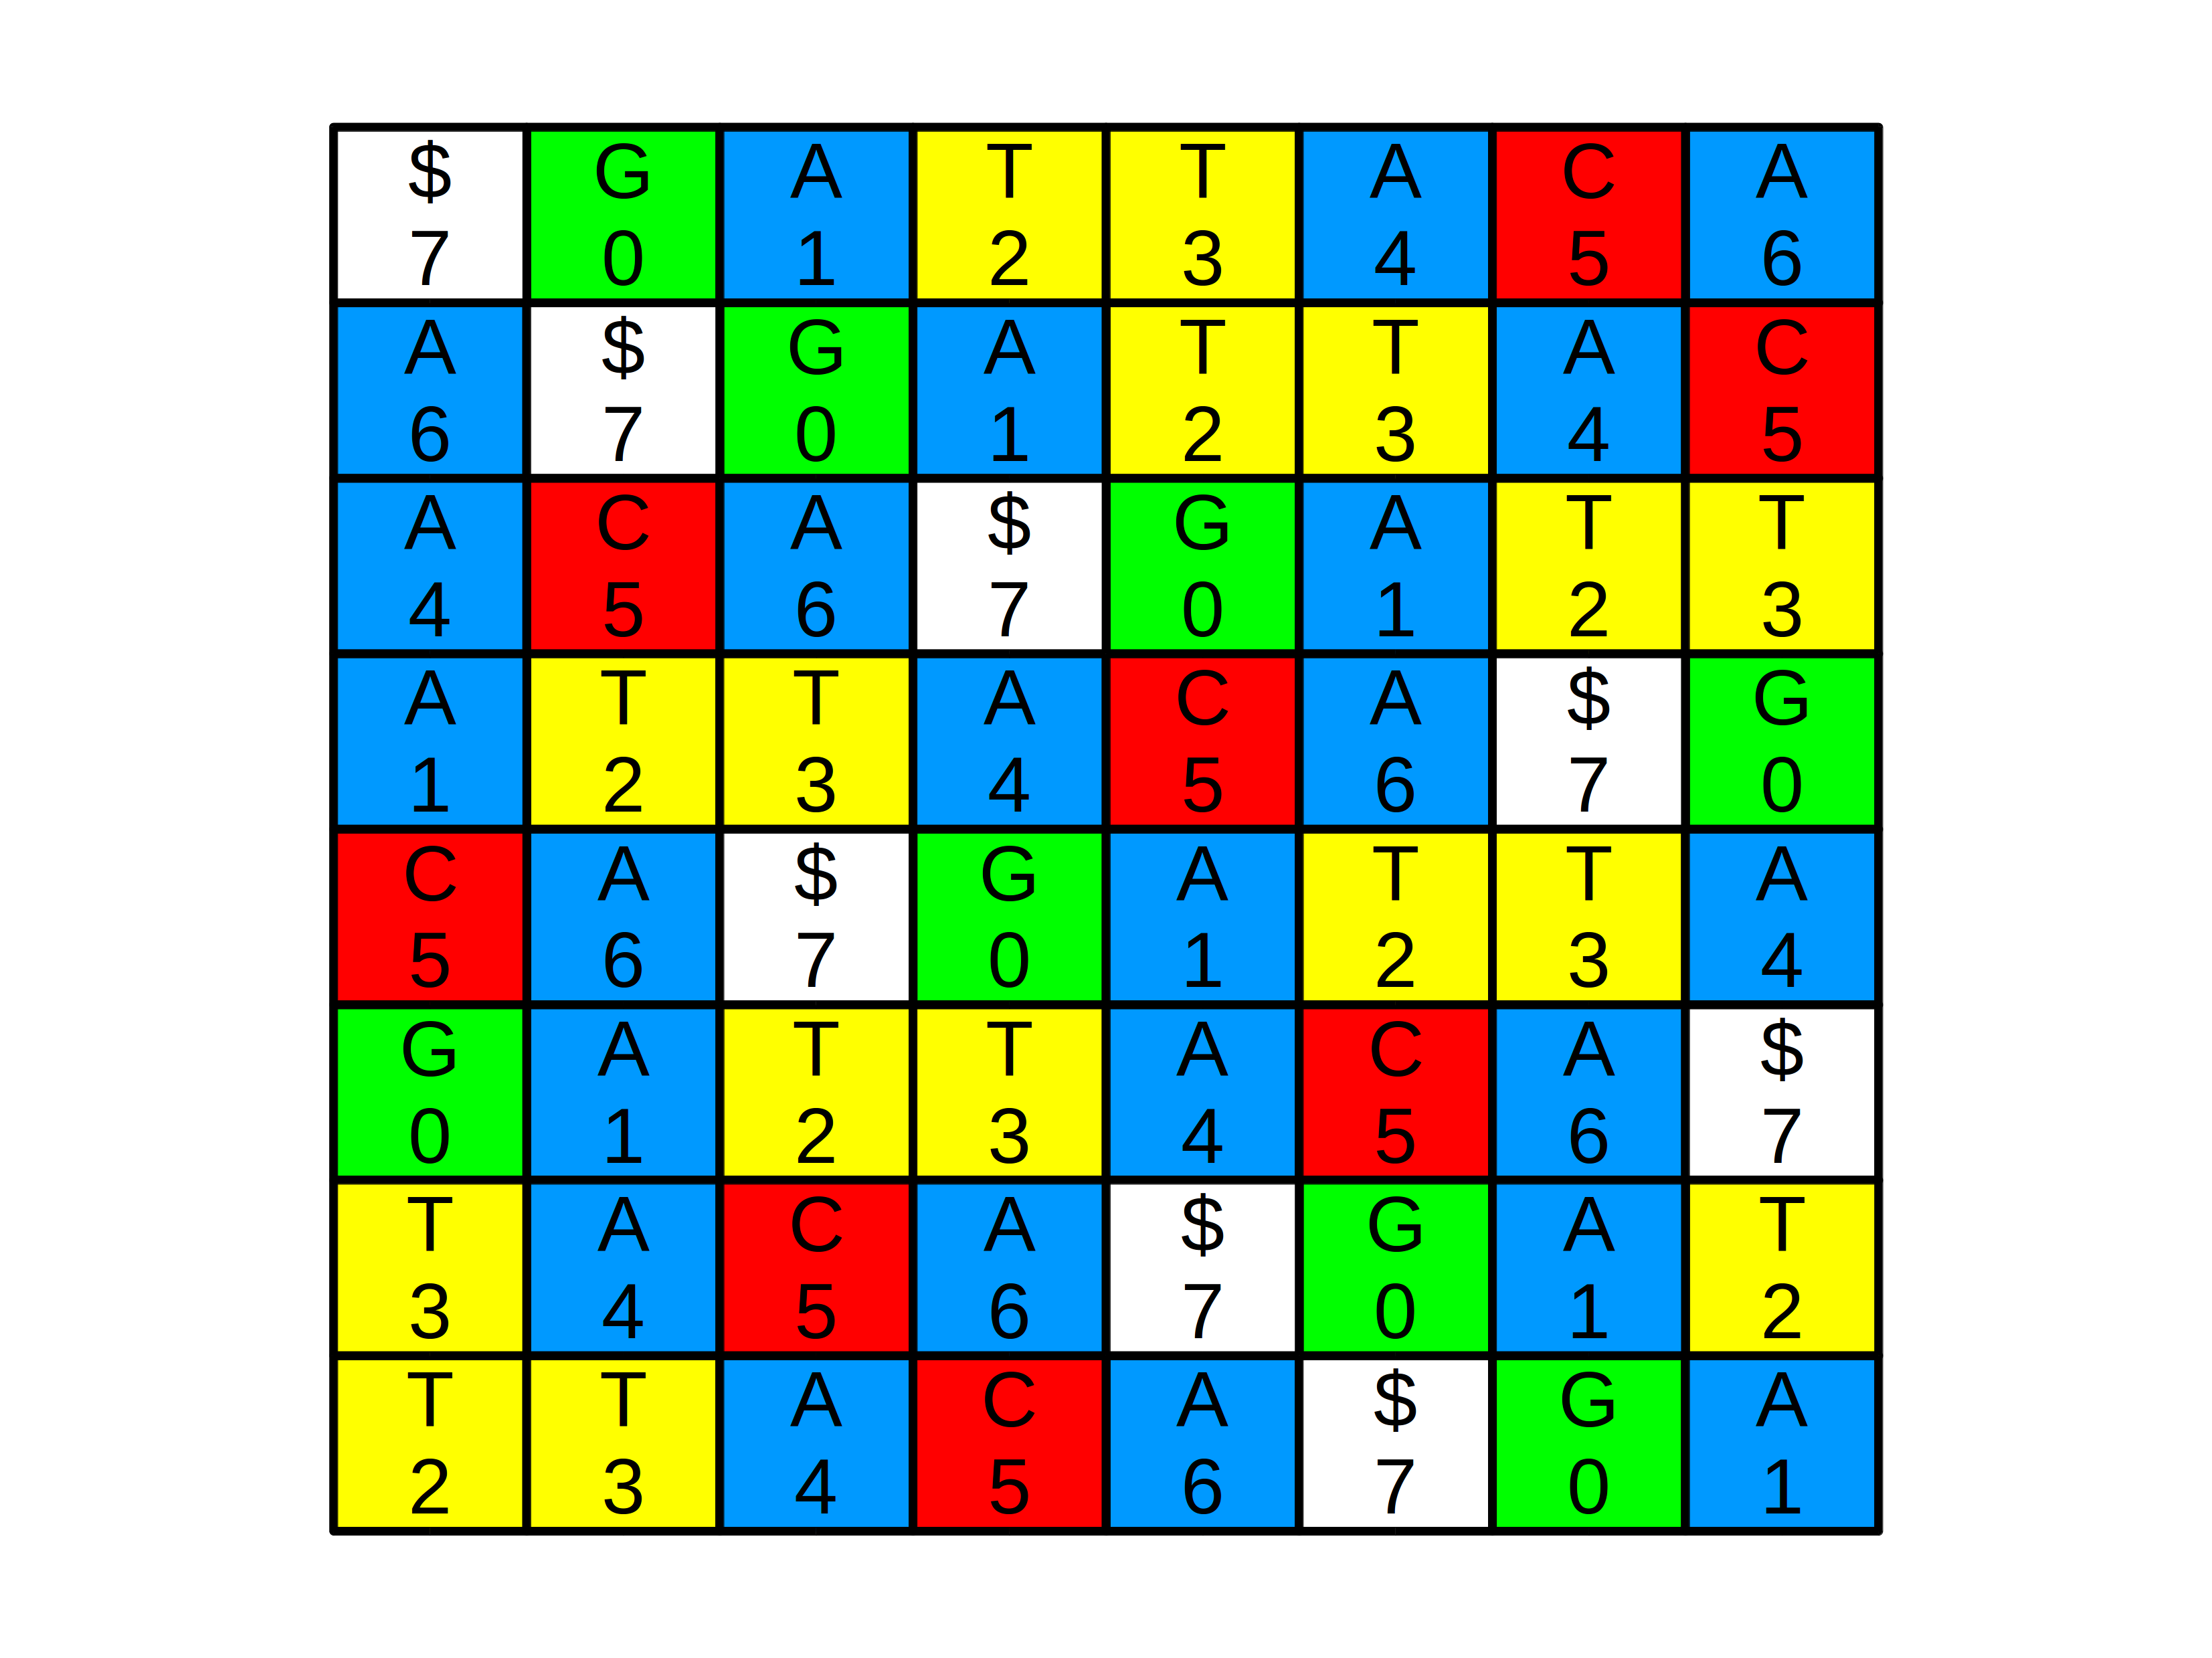
\includegraphics[width=1.0\textwidth]{figures/01_introduction/bwt.png}
    \caption[An example BWT matrix for the string ``GATTACA'']{An example BWT matrix for the string ``GATTACA''. The sentinel value ``\$'' is appended to the end of the string, all rotations of the string are calculated, and the rotations are sorted. Bases are colored according to base identity and numbered according to position in the original string. The characters in the far right column are the BWT of the original string, while the numbers in the far left column are the suffix array (represented as indices into the original string).}
    \label{fig:bwt}
\end{figure}

Note that the instances of any given character in the last column appear in the same relative order in the first column. Consider just the rows where the character in question appears in the first column. When sorting these rows, the first column is uninformative (since it is constant across all rows), and the rows are sorted lexicographically by the remaining columns in order. Rotating all the strings so the uninformative column appears last will not change the order of the other columns, and thus will not change the relative sort order of the rows we are considering. Thus the instances of the character stay in the same relative order in the last column as in the first column \cite{langmead2013introduction}.
    
\subsection{Substring Search with the Suffix Array}

The \vocab{suffix array} of a string is an array of indices into the string, sorted in the lexicographical order of the suffixes that they point to \cite{manber1993suffix}. For example, the string ``dog'' has suffixes ``dog'' at index 0, ``og'' at index 1, and ``g'' at index 2, so its suffix array would be $[0, 2, 1]$, corresponding to the suffix sort order $[\textrm{``dog''}, \textrm{``g''}, \textrm{``og''}]$. Another example suffix array is visible in the leftmost column of Figure~\ref{fig:bwt}.

Suffix arrays have some useful properties. Most importantly, all of the suffixes that start with the same substring appear in a single contiguous block \cite{ferragina2000opportunistic}. This block starts at the position corresponding to the number of occurrences of lexicographically smaller substrings of the same length \cite{ferragina2000opportunistic}. This is particularly obvious in the case of single-character substrings: all the suffixes (and, thus, all the substrings) beginning with a certain character appear in one block, coming immediately after all suffixes beginning with lexicographically smaller characters.

Suffix arrays can be used as indices to speed up substring search on the string they are derived from. Because of the block structure described above, and because every instance of a substring is at the beginning of some suffix, a simple binary search is sufficient to find any substring that is present, and a scanning up and down from one instance can pull out the entire corresponding block \cite{manber1993suffix}. Supplementing the suffix array with a \vocab{longest common prefix (LCP)} array, holding the length of the prefix shared by each pair of adjacent suffixes, can further speed up the search, by requiring only a single-character comparison (instead of a string comparison) at each search step \cite{manber1993suffix}.
    
\subsection{Searching in BWTs with the FM-index}

Constructing the BWT matrix is essentially the same task as constructing the suffix array of the string being transformed. All the rotations of the string contain the ``\$'' sentinel which is lexicographically less than all other characters. Thus the rotations are actually sorted by the portion before the ``\$'' character---that is, by the corresponding suffixes of the original string. This is the same sort used to construct the suffix array.

A BWT can be augmented with a small amount of additional information to create an FM-index (named after its inventors), which, like a suffix array, allows efficient substring search on the original string, but which also retains the compression afforded by the BWT \cite{ferragina2000opportunistic}. The FM-index is based primarily on the idea of an LF (i.e. last-first) mapping. This mapping maps each character instance in the last column of the BWT matrix to the row in which that same character instance appears in the first column. Because each BWT matrix row is a rotation of the original string, the last column of the row will contain the character instance immediately preceding the one just looked up. Thus, following the LF-mapping around the BWT from any starting position allows the characters of the original string to be enumerated from there in reverse order \cite{ferragina2000opportunistic}.

Since only the last column of the BWT matrix (i.e. the actual BWT string) is used in the algorithm, only that string needs to be stored. Furthermore, the LF-mapping can easily be calculated from the BWT string. To LF-map the character instance at a certain index in the BWT, count up the number of characters in the BWT lexicographically less than the character, and add the character instance's rank among all instances of that character. This gives the index of the LF-mapping result in the BWT.

To see why this works, recall that in a suffix array, and thus also in the BWT matrix, all the suffixes (or here rotations) that start with a given character form a contiguous block, coming just after all those beginning with smaller characters. Thus, the first calculation is to find the start of this block. And since, as shown in Subsection~\ref{subsec:bwt}, the relative order of character instances in the first column is the same as that in the last column, to find the offset of this particular character instance in that contiguous block, we merely need to find its rank among instances of the same character in the last column, which is the BWT string \cite{langmead2013introduction}.

We can now define \vocab{backward search}, a search algorithm using the BWT which processes the characters in the query string from back to front. The algorithm begins by selecting the entire BWT matrix, which is the range of suffixes that begin with the empty string. Then, for each character in the query string, from the last forwards, the algorithm extends the searched string at the front with that character. It takes the new character and finds the first and last instances of it in the BWT contained within the currently selected result range. It then LF-maps each of those instances, and takes the range between them as the new result range for the query string extended with that character. If there are no instances of the character to map, then the searched string is not found in the index \cite{ferragina2000opportunistic}.

Each row of the BWT matrix in the old range started with an instance of the old query string. Each of the rows that ended in the new query character corresponded to an instance of the old query string occurring after the new query character, and thus each implies an instance of the new, one-character-longer query string. The LF-mapping step finds the contiguous block of rows in the BWT matrix where those instances of the search string appear, the boundaries of which correspond to the first and last instances of the new character in the old BWT range (by the conservation of ordering mentioned at the end of Subsection~\ref{subsec:bwt}). Thus, such an algorithm can be used to search for substrings in a string, using the BWT of the string \cite{ferragina2000opportunistic}.

By pre-calculating some auxiliary data structures, such as a table with the start index of each character's range in the BWT matrix, and by using succinct data structures for $O(1)$ rank queries, this algorithm can be made to run in time linear in the length of the query string, and constant in the length of the index \cite{ferragina2000opportunistic}. Furthermore, using a downsampled copy of the suffix array, the location of each result in its source string can be calculated efficiently \cite{siren2009run}.

\subsection{Bidirectional DNA Search with the FMD-Index}

BWT-based indices have found many applications in genomics, mostly due to their ability to efficiently search for and identify the locations of a substrings in very large data sets---with a few modifications, this search can be extended to align reads to a reference \cite{li2014bwa}. The popular short read aligner \texttt{bwa}, for example, is built on an FM-index of the reference genome; indeed, the name stands for ``Burrows--Wheeler Aligner'' \cite{li2014bwa,li2009fast}. The ``String Graph Assembler'' \texttt{sga} also uses a BWT-based index to do its work, but in this case indexes reads themselves \cite{simpson2012efficient}.

In genomics, the strings being indexed are DNA strings, consisting of As, Gs, Cs, and Ts. These DNA strings are usually excerpts from double-stranded DNA genomes, in which, for each chromosome, two strands of DNA form a double helix. One strand runs in one direction, and the other strand runs in the other direction, with bases complemented (As and Ts swapped, and Gs and Cs swapped). It's impossible to tell whether a DNA sequencing read came from the forward strand or the reverse-complement strand until a match is found for it in a reference somewhere. Thus, many analysis problems in genomics need to consider not only some set of DNA strings but also their reverse complements.

The existence of reverse complements is accounted for in \texttt{sga} by creating two FM-indices of the input data: one index of the forward strand, and one of the reverse-complement strand \cite{simpson2012efficient}. This construction requires DNA query strings to be searched against both indices, and the results combined. However, there is a more elegant approach which allows the same search to be performed against a single index, and moreover allows bidirectional extension of the query string. This data structure, the ``FMD-index'' (the ``D'' is for ``DNA''), is simply an FM-index of both the forward and reverse strands of all input sequences, concatenated into a single data set \cite{li2012exploring}.

The FMD-index provides for double-ended search; that is, an intermediate search result can be extended with a character on either the left or right end of the query string. This works by having the FMD-index store as its intermediate result not just the single range in the BWT corresponding to BWT matrix rows that start with the query string, but also the (equally long) range for the reverse complement of the query string \cite{li2012exploring}. The first is the \vocab{forward range} and the second the \vocab{reverse range}. The fact that these two intervals will always be equally long is the key to the algorithm: because each string in the index is present as both itself and its reverse complement, any appearance of the query string has a corresponding appearance of its reverse complement. Extending the query string on the left causes the forward range to jump around in BWT coordinate space (to the regions of the BWT matrix that begin with the newly added character). However, extending on the left always causes the reverse range to cover a subrange of what it covered previously: the reverse complement of the query string gets extended on the right, and only BWT matrix rows which began with the original reverse-complement query string can possibly also begin with the longer reverse-complement query string.

The FMD-index search algorithm works as follows: When the query string is extended on the left, the forward range is updated as normal. The reverse range takes on the new interval length derived from the forward range, and a small dynamic programming problem is done over the alphabet to find its new start position. The dynamic programming problem is fairly simple because the reverse range can be partitioned into the ranges that would be selected upon left-extension with any character, ordered in lexicographic order by the reverse complement of the character. The dynamic programming simply consists of looping through the alphabet in lexicographic order by reverse complement, considering extending on each character up to the one actually being used, calculating how long the result set would be on the forward strand, and adding that in to the start of the reverse strand interval \cite{li2012exploring}. To extend a string on the right, the forward and reverse ranges are temporarily swapped, and the reverse complement of the query string is extended on its left with the reverse complement of the new base \cite{li2012exploring}.

\subsection{Previous Graph Indices}

% Improve this paragraph to actually say what is actually happening
The work that I am proposing involves implementing efficient search over graphs of genomic sequence data. This is not a new idea. Many of the current approaches to this problem come at it from the perspective of trying to index a multiple sequence alignment \cite{siren2014indexing}. Two such approaches are described below.

One approach, the Generalized Compressed Suffix Array (GCSA), extends the XBW transform (itself a generalization of the BWT to trees) to ``prefix-range-sorted automata'', which include de Bruijn graphs but not general directed labeled graphs \cite{siren2014indexing}. However, the authors of that approach present only an implementation for acyclic multiple sequence alignments. The existence of nonlinear structures like polymorphic inversions, where a genomic region is forwards in some individuals but backwards in others, is not addressed, and no implementation for de Bruijn graphs is provided \cite{siren2014indexing}. Moreover, the approach presented there provides search over all possible paths through the graph in question, which is a reasonable choice for indices derived from multiple alignments, but which might backfire for graphs with short cyclic structures that could provide pathological productions for many query strings \cite{siren2014indexing}.

Another, slightly newer approach uses the concept of a ``population reference graph'', also derived from a multiple sequence alignment \cite{dilthey2015improved}. In contrast to the BWT-based indexing methods described above, the population reference graph method turns its graph representation of genomes into a Hidden Markov Model (HMM), and identifies the most likely paths through it to match the k-mer spectrum of any particular sample \cite{dilthey2015improved}. Under this method, a pair of haploid genomes are then synthesized as sample-specific references, and existing read-to-genome mapping tools are used to map sequencing reads to these references \cite{dilthey2015improved}. Unfortunately, because of the way that k-mer counts from a sample are divided up to provide input for the HMM model in different genomic regions, this method is forced to divide its HMM states into ``levels'' that it proceeds through in a fixed, sequential order. The resulting graph model is constrained to closely resemble the multiple sequence alignment it was derived from. While this method can effectively model a wide range of alternative sequences in a region, it does not appear to be able to effectively model inversions, duplications, or other more complex structures \cite{dilthey2015improved}.

% Talk about and cite GCSA2 which actually gets used

% Maybe hit the vBWT as well

\section{Research Overview}

% Maybe this is where I should talk about tying together all the cools tuff I did and why I made the decisions I made

